\section{Auswertung}
\label{sec:Auswertung}
\paragraph{Bestimmung der Elementarladung}
Zur Bestimmung der Elementarladung wird zu erst die Gleichgewichtsgeschwindigkeit
$v_0$ berechnet, die Temperaturen im Kondensator und die daraus resultierende
Viskosität der Luft bestimmt. Danach wird die elektrische Feldstärke $E$ über
den Zusammenhang
\begin{equation*}
  E = \frac{U}{d}
\end{equation*}
bestimmt. Dabei bezeichnet $U$ die Spannung, die angelegt werden muss, dass der
beobachtete Öltropfen schwebt, $d$ bezeichnet den Abstand der Kondensatorplatten,
bei diesem Versuchsaufbau betrug der Abstand $d = \SI{7.6250(51)}{\milli\meter}$.
Aus den zuvor bestimmten Größen kann nun mit der Gleichung \eqref{eqn:rkorr}
der Radius des Öltropfen bestimmt werden, die Erdbeschleunigung
$g$ wird dabei aus \textit{Scipy-Physical Constants} \cite{scipy} entnommen, $\rho_{Oel}$ ist gegeben durch
\SI{886}{\kilo\gram\per\cubic\meter}. Alle Werte dazu sind in der Tabelle
\ref{tab:mill} dargestellt.
\begin{table}
  \centering
  \sisetup{round-mode = places , round-precision = 2}
         %rundet Werte aus Stelle, Stelle = ,  macht einen bestimmten festen exponenten
\resizebox{\textwidth}{!}{%
  \begin{tabular}{S S[scientific-notation=fixed, fixed-exponent= 0,round-precision=0] S[round-precision=3] S[round-precision = 6]@{$\quad\qquad\pm $} S S} % fügt plus minus Fehler Schreibweise hinzu
    \toprule
     $v_{0} / \si{\meter\per\second}$ & $T /\si{\celsius} $ & $\eta_{L} \cdot {10}^{5}/$ \si{\per\square\newton\second\meter}
     &\multicolumn{2}{c}{$r \pm \Delta r / \si{\meter}$}& $\text{E}/\si{\volt\per\meter}$\\
    \midrule
    4.816955684007706530e-05 & 2.900000000000000000e+01 & 1.863666666605290123e+00 & 2.014353871215394671e-04 & 2.149665866621864118e-12 & 5.901639344262294799e+03\\
    1.960553660353683895e-05 & 3.000000000000000000e+01 & 1.868166666603118253e+00 & 2.014347040396144320e-04 & 9.475290661159602373e-13 & 7.213114754098361118e+03\\
    2.010858636637844409e-05 & 3.000000000000000000e+01 & 1.868166666603118253e+00 & 2.014347161186670068e-04 & 9.718412356485277887e-13 & 7.213114754098361118e+03\\
    2.337213107091104457e-05 & 3.000000000000000000e+01 & 1.868166666603118253e+00 & 2.014347944817280556e-04 & 1.129566817444206731e-12 & 6.426229508196721326e+03\\
    4.014774369680424029e-05 & 3.000000000000000000e+01 & 1.868166666603118253e+00 & 2.014351972912206581e-04 & 1.940322355305905307e-12 & 3.921311475409835839e+04\\
    2.716948323642884541e-05 & 3.000000000000000000e+01 & 1.868166666603118253e+00 & 2.014348856623433869e-04 & 1.313090908517466980e-12 & 5.508196721311475812e+03\\
    2.920049056824154486e-05 & 3.000000000000000000e+01 & 1.868166666603118253e+00 & 2.014349344301231319e-04 & 1.411248387565193937e-12 & 2.531147540983606450e+04\\
    2.758316323716003923e-05 & 3.000000000000000000e+01 & 1.868166666603118253e+00 & 2.014348955954720338e-04 & 1.333083841676796001e-12 & 2.111475409836065592e+04\\
    2.997781641585227214e-05 & 3.100000000000000000e+01 & 1.872666666600946161e+00 & 2.014349548288511945e-04 & 1.559841162202571429e-12 & 1.206557377049180286e+04\\
    1.747396379394701858e-05 & 3.100000000000000000e+01 & 1.872666666600946161e+00 & 2.014346538677079534e-04 & 9.092272876084044865e-13 & 3.409836065573770611e+03\\
    2.401998462720983867e-05 & 3.100000000000000000e+01 & 1.872666666600946161e+00 & 2.014348114270358156e-04 & 1.249837109046131993e-12 & 1.731147540983606450e+04\\
    1.973476476160404450e-05 & 3.100000000000000000e+01 & 1.872666666600946161e+00 & 2.014347082840291204e-04 & 1.026863853047594021e-12 & 2.098360655737704747e+03\\
    2.392573452004976591e-05 & 3.300000000000000000e+01 & 1.881666666596603088e+00 & 2.014348119261527310e-04 & 1.422215226681806054e-12 & 1.665573770491803225e+04\\
    1.315789473684210598e-05 & 3.300000000000000000e+01 & 1.881666666596603088e+00 & 2.014345515041691926e-04 & 7.821445322221421246e-13 & 3.672131147540983875e+03\\
    2.246080589371546782e-05 & 3.300000000000000000e+01 & 1.881666666596603088e+00 & 2.014347764966317603e-04 & 1.335135844469047273e-12 & 1.600000000000000000e+04\\
    1.562158277876714722e-05 & 3.300000000000000000e+01 & 1.881666666596603088e+00 & 2.014346110889010894e-04 & 9.285932275608500287e-13 & 4.065573770491803316e+03\\
    1.559381237524949969e-05 & 3.300000000000000000e+01 & 1.881666666596603088e+00 & 2.014346104172690414e-04 & 9.269424754746385996e-13 & 4.196721311475409493e+03\\
    4.136333553937790236e-05 & 3.300000000000000000e+01 & 1.881666666596603088e+00 & 2.014352336566994017e-04 & 2.458751786403905334e-12 & 3.921311475409835839e+04\\
    2.552322613578356339e-05 & 3.300000000000000000e+01 & 1.881666666596603088e+00 & 2.014348505617226262e-04 & 1.517174482272390843e-12 & 9.704918032786885306e+03\\
    1.903601614254169181e-05 & 3.300000000000000000e+01 & 1.881666666596603088e+00 & 2.014346936675479450e-04 & 1.131556813089161264e-12 & 1.350819672131147490e+04\\
    1.644682740699319220e-05 & 3.300000000000000000e+01 & 1.881666666596603088e+00 & 2.014346310475847209e-04 & 9.776481198068857039e-13 & 2.662295081967213264e+04\\
    1.667945424825699761e-05 & 3.300000000000000000e+01 & 1.881666666596603088e+00 & 2.014346366737046251e-04 & 9.914761203685482155e-13 & 3.947540983606557711e+04\\
    1.447722732142340251e-05 & 3.300000000000000000e+01 & 1.881666666596603088e+00 & 2.014345834124637484e-04 & 8.605694622390387846e-13 & 1.009836065573770429e+04\\
    1.817520901490366975e-05 & 3.300000000000000000e+01 & 1.881666666596603088e+00 & 2.014346728487855409e-04 & 1.080388016131123836e-12 & 3.803278688524590052e+03\\
    3.136172614940726681e-05 & 3.300000000000000000e+01 & 1.881666666596603088e+00 & 2.014349917666419113e-04 & 1.864230526082146843e-12 & 1.324590163934426346e+04\\
    1.240048609905508317e-05 & 3.300000000000000000e+01 & 1.881666666596603088e+00 & 2.014345331861035139e-04 & 7.371219693636488841e-13 & 7.213114754098361118e+03\\
    1.923816852635629282e-05 & 3.300000000000000000e+01 & 1.881666666596603088e+00 & 2.014346985566363738e-04 & 1.143573317867085913e-12 & 1.613114754098360754e+04\\
    1.583932587829061888e-05 & 3.300000000000000000e+01 & 1.881666666596603088e+00 & 2.014346163550556807e-04 & 9.415364988019333343e-13 & 3.947540983606557711e+04\\
    2.205655300189686215e-05 & 3.300000000000000000e+01 & 1.881666666596603088e+00 & 2.014347667197131735e-04 & 1.311105936565683071e-12 & 5.770491803278689076e+03\\
    5.862351975612615671e-05 & 3.300000000000000000e+01 & 1.881666666596603088e+00 & 2.014356510955293237e-04 & 3.484737954539736415e-12 & 1.468852459016393550e+04\\
    \bottomrule
  \end{tabular}
}
  \caption{Wert zur Berechnung der Ladungsmenge, auf einem Öltropfen. Dabei
  bezeichnet \texorpdfstring{$v_0$}{math} die Gleichgewichtsgeschwindigkeit, T
  die Temperatur im Kondensator, r den Radius des Öltropfens und E die elektrische
  Feldstärke im Kondensator.}
  \label{tab:mill}
\end{table}
\FloatBarrier
Da nun alle Größen bestimmt wurden die in der Gleichung \eqref{eqn:q} benötigt
werden, kann die Ladung die auf den Öltropfen bestimmt werden, die Erdbeschleunigung
$g$ wird dabei aus \textit{Scipy-Physical Constants} \cite{scipy} entnommen, $\rho_{Oel}$ ist gegeben durch
\SI{886}{\kilo\gram\per\cubic\meter}. Die Werte
der Ladung und des Radius der Öltropfen werden nach der größe sortiert und dann
wird die Ladung gegen den Radius aufgetragen. Das ist in Abbildung \ref{fig:eQ}
dargestellt. In besagter Abbildung können dann Niveaus beobachtet werden, die
Vielfache der Elementarladung darstellen. Die Ladungsmengen auf diesen Niveaus
werden dann gemittelt. In der Abbildung \ref{fig:eQ} sind zwei Niveaus zu
beobachten. Daraus lässt sich dann wie folgt die Elementarladung bestimmen:
\begin{equation*}
  q = \frac{\bar{q}_{Niveau 1} + \frac{1}{2}\cdot \bar{q}_{Niveau2}}{2} \; .
\end{equation*}
Mit den Mittelwerten $q_{Niveau1} = \SI{1.822(7)e-19}{\coulomb}$ und
$ q_{Niveau2} = \SI{2.053(8)e-19}{\coulomb}$, ergibt sich für die
Elemntarladung $q = \SI{1.424(5)e-19}{\coulomb}$.
\begin{figure}
  \centering
  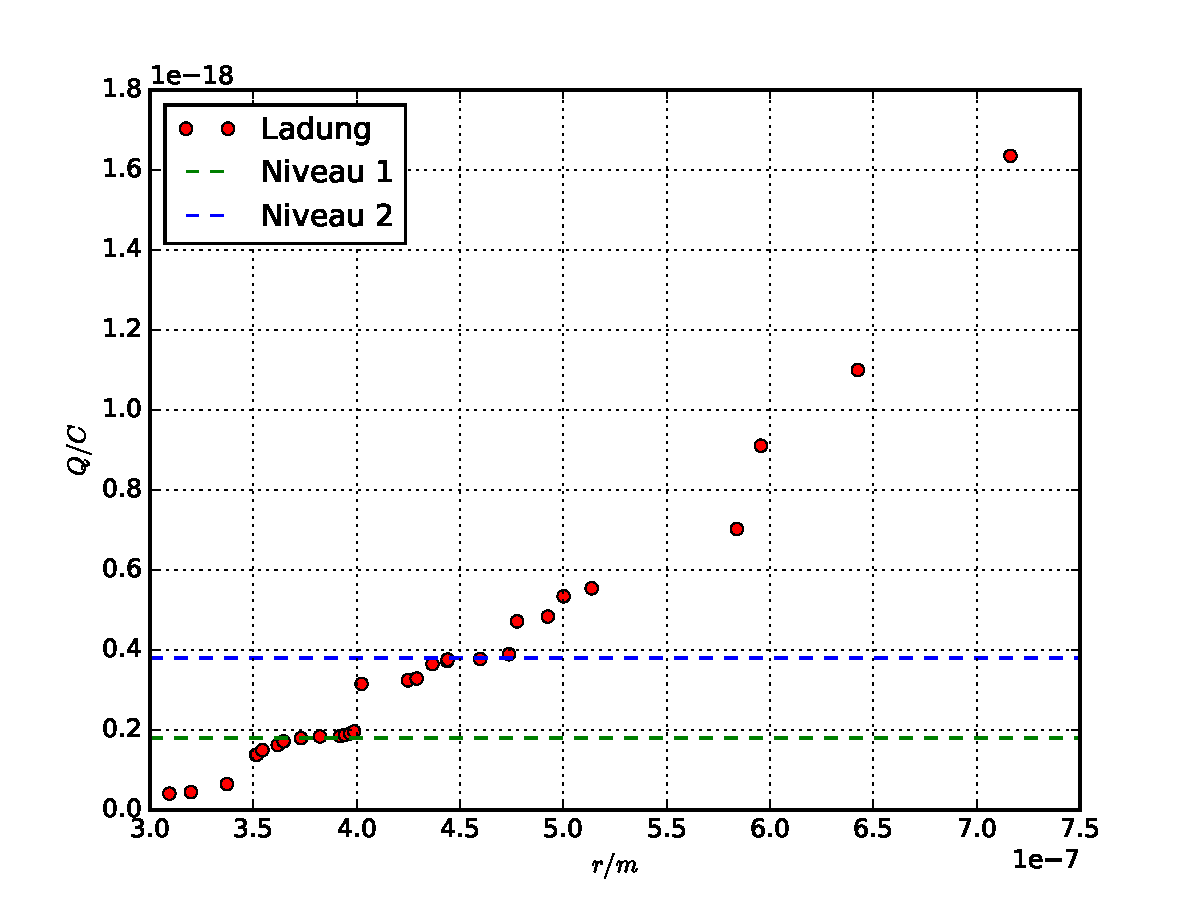
\includegraphics[height=7cm]{plots/milliplot.pdf}
  \caption{In dieser Darstellung sind die gemessene Ladung,
  auf den Öltropfen, gegen den Radius, des Öltropfen, aufgezeichnet.}
  \label{fig:eQ}
\end{figure}
\FloatBarrier
\paragraph{Bestimmung der Avogadro-Konstante}
Die Avogadro-Konstante ergibt sich mit der \textit{Faraday-Konstante} \cite{scipy}
durch den Zusammenhang
\begin{equation*}
  N_{A} = \frac{\symup{F}}{e_0} = \frac{\symup{F}}{q} \; .
\end{equation*}
Für die zuvor bestimmte Elementarladung ergibt sich die Avogadro-Konstante
$N_A = \SI{6.78(2)e23}{\per\mol}$.
























%
